\documentclass[border=3pt]{standalone}
\usepackage{tikz}
\usetikzlibrary{arrows.meta,calc,positioning}
\tikzset{pin/.style={-{Stealth[length=5pt]}},
  blk/.style={draw, thick, minimum width=15mm, minimum height=11mm, font=\sffamily\small, align=center}}
\begin{document}
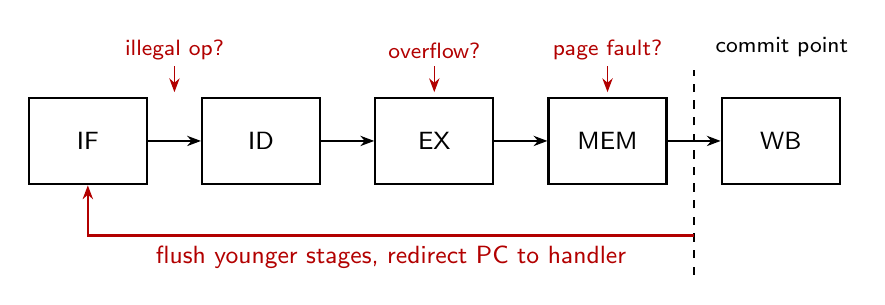
\begin{tikzpicture}[font=\sffamily\small]
  \node[blk] (if)  at (0,0)   {IF};
  \node[blk] (id)  at (2.2,0) {ID};
  \node[blk] (ex)  at (4.4,0) {EX};
  \node[blk] (mem) at (6.6,0) {MEM};
  \node[blk] (wb)  at (8.8,0) {WB};
  \foreach \a/\b in {if/id, id/ex, ex/mem, mem/wb}{\draw[pin] (\a.east) -- (\b.west);}
  % exception flags ride along
  \node[font=\sffamily\footnotesize, red!70!black] at (1.1,1.15) {illegal op?};
  \node[font=\sffamily\footnotesize, red!70!black] at (4.4,1.15) {overflow?};
  \node[font=\sffamily\footnotesize, red!70!black] at (6.6,1.15) {page fault?};
  \foreach \x in {1.1,4.4,6.6}{\draw[pin, red!70!black] (\x,0.95) -- (\x,0.62);}
  % commit point
  \draw[thick, dashed] (7.7,-1.7) -- (7.7,0.9);
  \node[font=\sffamily\footnotesize, anchor=south west] at (7.85,0.95) {commit point};
  % flush arrows
  \draw[pin, red!70!black, thick] (7.7,-1.2) -| node[below, pos=0.25]{flush younger stages, redirect PC to handler} (if.south);
\end{tikzpicture}
\end{document}
